\documentclass[../Bachelorarbeit.tex]{subfiles}
\begin{document}

\graphicspath{{./figures/theory/nw/}}	%specifying the folder for the figures

\section{Complex Networks}
\label{sec:theory_complexNetworks}
Networks play an important role in trading-processes and in the context of double auctions as they define which trader is able to interact with others thus influencing the process fundamentally. This thesis lays its main focus on the influence of network-topologies on the equilibrium found in continuous double-auction. The networks define the neighbourhood between agents and determine which pair of agents can trade with each other. All graph-related definitions in the following sections are provided through \cite{Drmota2007}.

\medskip

A network is a graph \textit{G = (V,E)} which has a finite set of vertices \textit{V = V(G)} and a finite set of edges \textit{E = E(G)}. The vertices represent the agents and the edges connecting them represent the neighbourhood between agents or the knowledge of each other. Two agents know each other and can trade with each other if there exists an edge between them. In this context only undirected graphs consisting of undirected edges $e$ $\in$ $E(G)$, $e = {v_1, v_2}$ between two vertices $v_1$, $v_2$ $\in$ $V(G)$ without multi- and self-edges are of interest.

\begin{itemize}
\item Undirected: if one agent $v_1$ knows another agent $v_2$ then $v_2$ knows $v_1$ too - trading is always possible in both directions.
\item No multi-edges: one neighbourhood connection is enough as edges have no additional properties or weights.
\item No self-edges: agents are not allowed to trade with themselves.
\end{itemize}

This thesis also investigates the equilibrium in so called \textit{complex networks} which are a special kind of random network which could exhibit small-world properties and could follow a power-law distribution which are discussed below. In the following sections a short overview of the development of network-topologies and recent findings in this research-field is given and the complex networks used in this thesis are discussed. See appendix \ref{app:topologies} for a complete catalogue of network-topologies investigated in this thesis - the complex ones are:

\begin{itemize}
\item Erdos-Renyi
\item Barbasi-Albert
\item Watts-Strogatz
\end{itemize}

The main sources for the following sections is the paper \cite{Newman_ComplexNetworks} and the books \cite{Jackson2008} and \cite{Easley2010}. Note that in this thesis only static networks are of interest thus no models of network-growth or processes in and on networks are discussed.

\subsection{Overview}
Since the first proof in network-theory by Euler in 1735 the analysis of networks has had a long tradition. Up until a few years ago the analysis of small graphs and properties of individual vertices or edges dominated the field of network-research, but in recent years the focus shifted towards large-scale statistical properties. This transition of focus was made possible by the availability of an ever increasing amount of processing power through computers which allow the investigation of networks with millions of vertices.

\subsection{Random graphs}
One of the simplest network models studied was the random graph which was investigated first by \cite{ErdosRenyi1959}. The motivation behind random graphs is to assume a random-process of network formation and to study the resulting networks. Such networks are constructed by having \textit{N} unconnected vertices and then adding at random each possible edge with a given probability \textit{p} where the distribution of \textit{p} follows a specific model, e.g. uniform, poisson, gaussian and so on. Thus random graphs can be reduced to a "binomial model of link formation" \cite{Jackson2008} where out of all the possible random graphs with \textit{N} nodes one graph is selected with a probability of 

\begin{equation}
p^m(1-p) \frac{N(N-1)}{2} - m
\end{equation}

as reported in \cite{Jackson2008}.

\subsection{Small-World effects}
In the 1960s Stanley Milgram conducted an experiment in which he demonstrated that a letter can reach any destination person by an average of just 6 intermediate steps in between. In his papers on this experiment \cite{TraverMilgram_StudySmallWorld} and \cite{Milgram_SmallWorld}, he termed this phenomenon the \textit{small-world effect}. Although the results of his work have been questioned - more specifically that the world is really a small one e.g. by \cite{Kleinfeld_BigWorld} - it had big influences within the network-research community and led to the development of the small-world property. It is of great importance e.g. in social networks because this property implies that information spreads very quickly in the network as it needs very few steps to reach all nodes. This can also be applied to trading networks where it enables traders to trade goods within very few intermediary steps to traders which value the goods the most.

\medskip

To calculate whether a network has the small-world property, one starts with the formula given by \cite{Newman_ComplexNetworks} for calculating the average path length in a network

\begin{equation}
\ell = \frac{1}{\frac{1}{2}N(N+1)} \displaystyle\sum_{i \geq j }^{} d_{ij}
\end{equation}

where $d_{ij}$ is the shortest distance from vertex i to vertex j. Networks then exhibit the small-world property if $\ell$ scales at max logarithmically with network size of mean degree.

\subsection{Scale-free networks}
\cite{BarabasiAlbert_EmergenceScaling} found that real-world networks in contrast to random graphs are non-random which led to the discovery of the phenomena of scale-free networks which are networks whose vertex-degree distribution follows a power-law as defined below.

\subsubsection{Degree distribution}
In an undirected Graph \textit{G} the edges adjacent to $v$ $\in$ $V(G)$ 

\begin{equation}
\Gamma(v) = {w \in V(G) | vw \in E(G)}
\end{equation}

are the neighbours. The quantity of the neighbours of $v$ $\in$ $V(G)$ 

\begin{equation}
d(v) = |\Gamma(v)| = |{w \in V(G) | vw \in E(G)}|
\end{equation}

is the degree of a vertex $v$ $\in$ $V(G)$. When regarding the adjacent-matrix of a graph the degree of a vertex $v_i$ $\in$ $V(G)$ is given by

\begin{equation}
d(v_i) = \displaystyle\sum_{j=1}^{n} a_{ij}
\end{equation}

Having defined the degree of a vertex one can calculate the degree distribution of of a given network simply by counting the number of nodes which have a given degree k:

\begin{equation}
P_{deg}(k) = \textit{fraction of nodes in the graph with degree k}
\end{equation}

\begin{figure}[H]
	\centering
  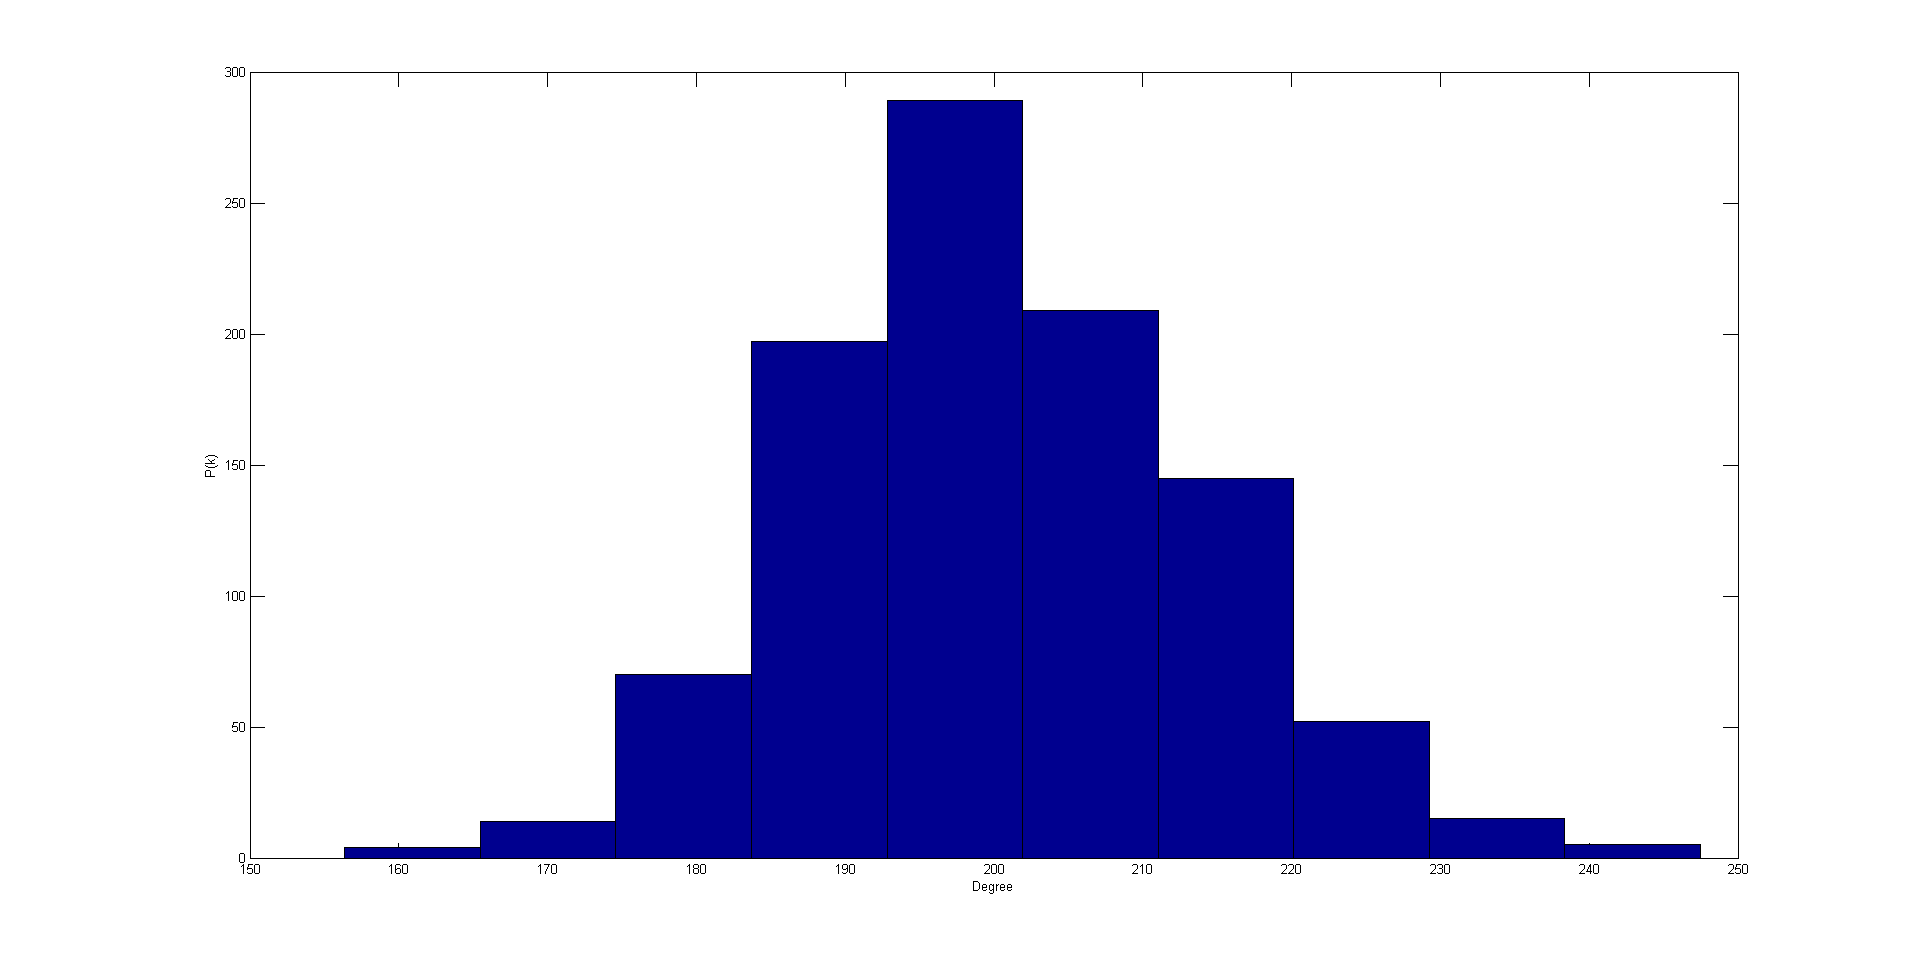
\includegraphics[width=1.0\textwidth, angle=0]{ERDOSRENYI_DEGREE_HIST.png}
  	\caption{Histogram of the degree-distribution of a random Erdos-Renyi network with 1000 agents generated by the thesis-software. The average degree is 200.44.}
	\label{fig:ERDOSRENYI_DEGREE_HIST}
\end{figure}

\subsubsection{Power-law distribution}
In figure \ref{fig:BARBASIALBERT_HIST} the degree-distribution of a scale-free network is shown.

\begin{figure}[H]
	\centering
  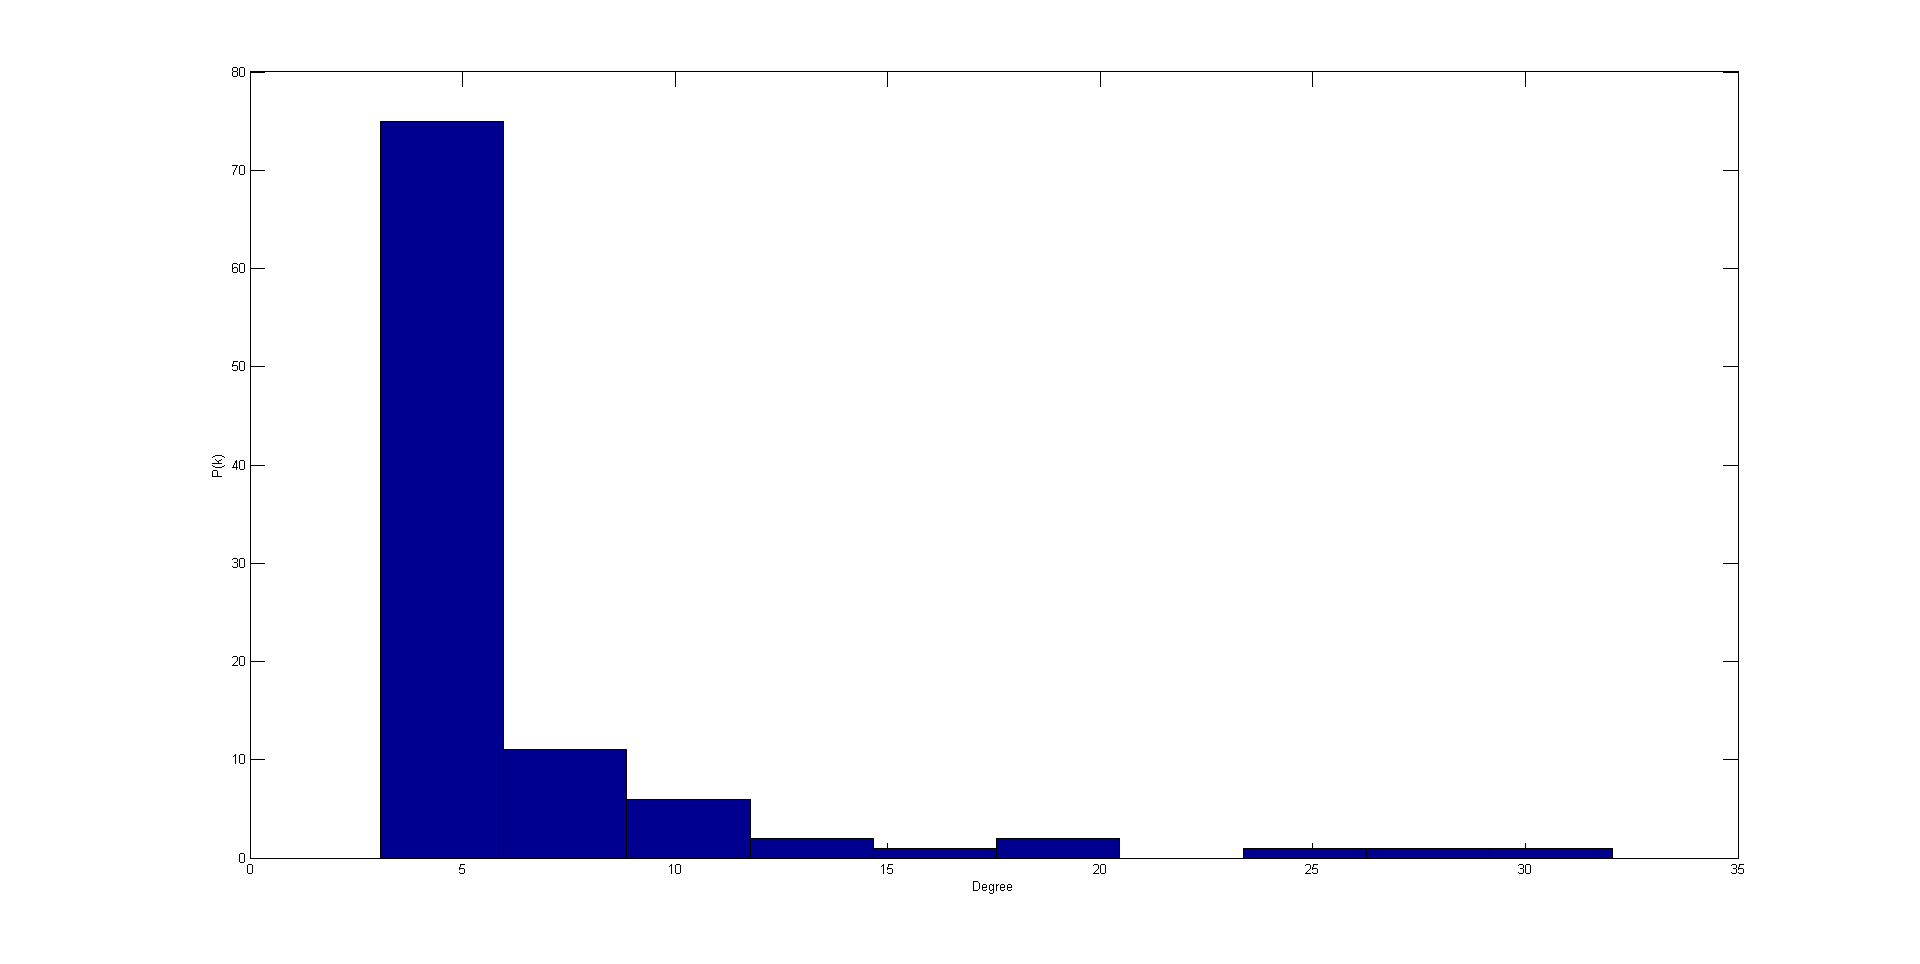
\includegraphics[width=1.0\textwidth, angle=0]{BARBASIALBERT_HIST.png}
  	\caption{Histogram of the degree-distribution of a Barbasi-Albert network with 100 agents generated by the thesis-software. The average degree is 4.1. Note that the Barbasi-Albert model creates scale-free networks.}
	\label{fig:BARBASIALBERT_HIST}
\end{figure}

What is striking about figure \ref{fig:BARBASIALBERT_HIST} is the long right tail. This shows that there exist few vertices in this network which have a very high degree far beyond the average degree. This means that many other vertices are connected to them - they act as a kind of hub. Most of the vertices though have a low degree around 5 which in combination with the few high-degree vertices results in the long tail of this distribution which follows a power-law

\begin{equation}
P_{deg}(k) \sim k^{-\gamma}
\end{equation}

Note that due to the power-law the distribution of such networks remain unchanged when scaling \textit{k} with a given factor \textit{a}. Thus those networks are called \textit{scale-free}.

\begin{figure}[H]
	\centering
  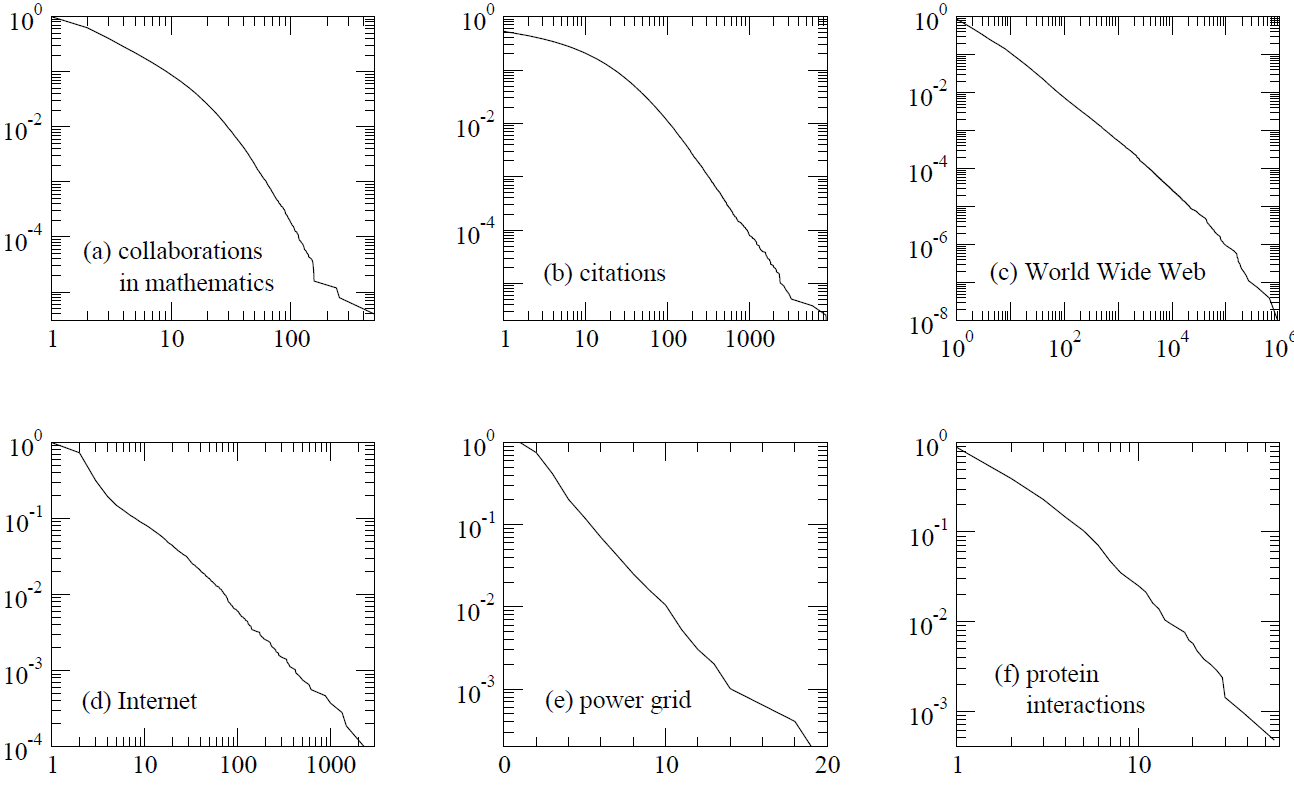
\includegraphics[width=1.0\textwidth, angle=0]{SCALEFREE_REALWORLD_EXAMPLES.png}
  	\caption{Examples for degree-distributions of real-world networks. Note that a straight line in a log-log plot is evidence of a power-law distribution thus only (c), (d) and (f) appear to have power-law distributions. \cite{Newman_ComplexNetworks} }
	\label{fig:SCALEFREE_REALWORLD_EXAMPLES}
\end{figure}

\medskip

The strengths of scale-free networks is their resilience against \textit{random} removal of vertices.

\begin{figure}[H]
	\centering
  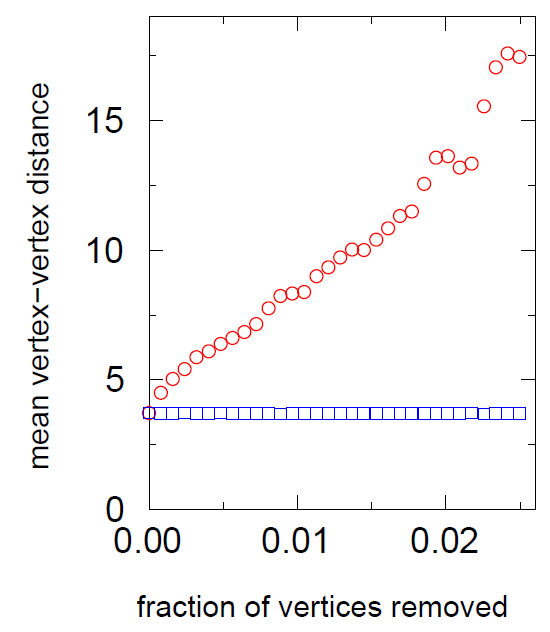
\includegraphics[width=0.5\textwidth, angle=0]{RESILIENCE.png}
  	\caption{Random removal of vertices increases the average path length very slightly. Removing vertices with highest degree first increases the average path length rapidly. \cite{Newman_ComplexNetworks} }
	\label{fig:RESILIENCE}
\end{figure}

This resilience can be of benefit in a scale-free trading network where the inability of a random trader to trade because it has no more goods or cash won't impair the overall trading ability. On the other hand if an important trader which acts as a hub becomes unable to trade then the overall trading process may be affected.

\subsection{Complex Network examples}
To summarize complex networks are random networks that could have small-world properties and could be scale-free depending on the algorithms used to create them. There exist a few models to create complex networks where three well known models are implemented in this thesis. See appendix \ref{app:topologies} for examples of the following networks created by the thesis-software with varying parametrization.

\subsubsection{Erdos-Renyi}
The Erdos-Renyi model generates a pure random-graph which exhibits \textit{no} small-world properties. It starts with \textit{N} vertices and selects one out of all the possible graphs with \textit{n} vertices by random iteration over all possible edges and including each with a given probability \textit{p}. \cite{ErdosRenyi1959} and \cite{ErdosRenyi_EvolutionRandomGraphs}

\subsubsection{Watts-Strogatz}
The Watts-Strogath model generates a random-graph which exhibits small-world properties. It starts with \textit{N} unconnected vertices and creates a regular lattice where each vertex is connected to \textit{K} neighbours with $\frac{K}{2}$ on each side. It then iterates through all vertices and and rewires each edge which is connected to a vertex already visited with a given probability \textit{b} to another vertex from all the possible vertices - self-loops and link-duplication is not allowed. \cite{WattsStrogatz_DynamicsSmallWorld}

\subsubsection{Barbasi-Albert}
The Barbasi-Albert model generates a random-graph which exhibits small-world and scale-free properties which is achieved through preferential attachment. To create a network with \textit{N} vertices one starts with $m_0$ vertices and adds $N - m_0$ vertices. Each new vertex is connected to \textit{m} existing vertices where the probability to be connected to a given vertex is proportional to its degree. When choosing m = 1 then one creates a hub-structure. \cite{BarabasiAlbert_EmergenceScaling}

\end{document}